\documentclass[14pt,aspectratio=1610]{beamer}

\usepackage[brazil]{babel}
\usepackage[utf8]{inputenc}
%\UseRawInputEncoding
\usepackage[T1]{fontenc}
\usepackage{Sweave}
\usepackage{animate}
\usepackage{amsbsy}
\usepackage{amsfonts}
\usepackage{amsmath}
\usepackage{amssymb}
\usepackage{amsthm}
\usepackage[toc,page,title,titletoc]{appendix}
\usepackage[fixlanguage]{babelbib}
%\usepackage[pdftex]{color}
\usepackage{dsfont}
\usepackage{esvect}
\usepackage[labelfont=bf]{caption}
\usepackage{float}
\usepackage[Glenn]{fncychap}%Sonny %Conny %Lenny %Glenn %Renje %Bjarne %Bjornstrup
%\usepackage{geometry, calc, color, setspace}%
%\geometry{a4paper, headsep=1.0cm, footskip=1cm, lmargin=3cm, rmargin=2cm, tmargin=3cm, bmargin=2cm}
\usepackage{graphicx}
\usepackage{indentfirst}%Para indentar os parágrafos automáticamente
\usepackage{lipsum}
\usepackage{longtable}
\usepackage{mathtools}
\usepackage{listings}%Inserir codigo do R no latex
\usepackage{multirow}
\usepackage{multicol}
\usepackage{natbib}
\bibliographystyle{abbrvnat3}
\usepackage[figuresright]{rotating}
\usepackage{spalign}
%\usepackage{pgfpages}
\usepackage{pgfplots}
\usepackage{tikz}
\usepackage{color, colortbl}
\usepackage{ragged2e}%para justificar o texto dentro de algum ambiente
\definecolor{Gray}{gray}{0.9}
\definecolor{LightCyan}{rgb}{0.88,1,1}


\usepackage[all]{xy}
\usepackage{hyperref,bookmark}
\hypersetup{
  colorlinks=true,
  linkcolor=blue,
  citecolor=red,
  filecolor=blue,
  urlcolor=blue,
}

\usetheme{JuanLesPins}
\usecolortheme[RGB={193,0,0}]{structure}

%\setbeamertemplate{footline}[frame number]
%\setbeamertemplate{footline}[text line]{%
%  \parbox{\linewidth}{\vspace*{-8pt}\hfill\date{}\hfill\insertshortauthor\hfill\insertpagenumber}}
\beamertemplatenavigationsymbolsempty
\renewcommand{\vec}[1]{\mbox{\boldmath$#1$}}
\newtheorem{Teorema}{Teorema}
\newtheorem{Proposicao}{Proposição}
\newtheorem{Definicao}{Definição}
\newtheorem{Corolario}{Corolário}
\newtheorem{Demonstracao}{Demonstração}
\newcommand{\bx}{\ensuremath{\bar{x}}}
\newcommand{\Ho}{\ensuremath{H_{0}}}
\newcommand{\Hi}{\ensuremath{H_{1}}}

\newcounter{saveenumi}
\newcommand{\seti}{\setcounter{saveenumi}{\value{enumi}}}
\newcommand{\conti}{\setcounter{enumi}{\value{saveenumi}}}

\apptocmd{\frame}{}{\justifying}{} % Allow optional arguments after frame.

\title{MAF 105 - Estatística Básica}
\author{Prof. Fernando de Souza Bastos}
\institute{Instituto de Ciências Exatas e Tecnológicas\texorpdfstring{\\ Universidade Federal de Viçosa}{}\texorpdfstring{\\ Campus UFV - Florestal}{}}
\date[\today]{}
\newcommand\mytext{Aula 2}
\newcommand\mytextt{Fernando de Souza Bastos}
\makeatletter
\setbeamertemplate{footline}
{
  \leavevmode%
  \hbox{%
  \begin{beamercolorbox}[wd=.333333\paperwidth,ht=2.25ex,dp=1ex,center]{author in head/foot}%
    \usebeamerfont{author in head/foot}\mytext
  \end{beamercolorbox}%
  \begin{beamercolorbox}[wd=.333333\paperwidth,ht=2.25ex,dp=1ex,center]{title in head/foot}%
    \usebeamerfont{title in head/foot}\mytextt
  \end{beamercolorbox}%
  % \begin{beamercolorbox}[wd=.333333\paperwidth,ht=2.25ex,dp=1ex,right]{date in head/foot}%
  %   \usebeamerfont{date in head/foot}\insertshortdate{}\hspace*{2em}
  %   \insertframenumber{} / \inserttotalframenumber\hspace*{2ex} 
  % \end{beamercolorbox}
  }%
  \vskip0pt%
}
\makeatother


\providecommand{\arcsin}{} \renewcommand{\arcsin}{\hspace{2pt}\textrm{arcsen}}
\providecommand{\sin}{} \renewcommand{\sin}{\hspace{2pt}\textrm{sen}}
%\newtheorem{Teorema}{Teorema}
%\newtheorem{Proposicao}{Proposição}
%\newtheorem{Definicao}{Definição}
%\newtheorem{Corolario}{Corolário}
%\newtheorem{Demonstracao}{Demonstração}

% Layout da pagina
\hypersetup{pdfpagelayout=SinglePage}
\begin{document}
\Sconcordance{concordance:Aula2.tex:Aula2.Rnw:%
1 252 1}


\frame{\titlepage}

\begin{frame}{}
\frametitle{\bf Sumário}
\tableofcontents
\end{frame}

\section{Somatórios}
\begin{frame}{}
\frametitle{Somatório}
\begin{block}{}
\justifying
O somatório é uma forma abreviada para representação de somas. Podemos defini-lo como o operador matemático para a soma dos termos de uma sequência. Usualmente, um somatório é representado pela letra grega sigma maiúscula $(\Sigma)$ e é definido por:
\begin{equation}
{\displaystyle \sum_{i=m}^{n}x_{i}=x_{m}+x_{m+1}+\cdots+x_{n}.}
\end{equation}
em que $\{ x_{k} \}_{k\in \mathds{N}}$ é uma sequência dada, $i$ é o índice do somatório, $m$ denota o limite inferior e $n$ o limite superior.
\end{block}
\end{frame}

\begin{frame}{}
\frametitle{Somatório}
\begin{block}{}
\justifying
Como exemplo note que
\begin{equation}
{\displaystyle \sum_{i=1}^{n}x_{i}=1+2+3+\cdots+(n-2)+(n-1)+n}
\end{equation}
Se lê: ``Soma de $i,$ para $i=1$ até $n.$''
\end{block}
\pause
\begin{block}{}
\justifying
ou,
\begin{equation}
{\displaystyle \sum_{i=0}^{k}(2i+1)=1+3+\cdots+(2k-1)+(2k+1)}
\end{equation}
que se lê: ``Soma de $(2i+1),$ para $i=0$ até $k.$''
\end{block}
\end{frame}

\begin{frame}{}
\frametitle{Propriedades}
\begin{block}{}
\justifying
\begin{enumerate}
\item ${\displaystyle \sum_{i=m}^{n}ax_{i}=a\sum_{i=m}^{n}ax_{i}\ \forall a\in \mathds{R}, m,n\in \mathds{Z}.}$
\item ${\displaystyle \sum_{i=m}^{n}K=[(n-m)+1]K},$ $K$ constante real qualquer. Em particular para $m=1,$ temos 
${\displaystyle \sum_{i=1}^{n}K=nK}.$
    \seti
\end{enumerate}
\end{block}
\end{frame}

\begin{frame}{}
\frametitle{Propriedades}
\begin{block}{}
\justifying
\begin{enumerate}
    \conti
\item ${\displaystyle \sum_{i=m}^{n}(a_{i}x_{i}+b_{i}z_{i})=\sum_{i=m}^{n}(a_{i}x_{i})+
\sum_{i=m}^{n}(b_{i}z_{i}),\ \forall m,n\in \mathds{Z}.}$ 
\item ${\displaystyle \sum_{i=k}^{n}(x_{i}-x_{i+1})=x_{k}-x_{n+1}}$  
\item ${\displaystyle \sum_{k=0}^{n}K=\sum_{k=1}^{n}K=\dfrac{n(n+1)}{2}}$ (Soma de Gauss) 
    \seti
\end{enumerate}
\end{block}
\end{frame}

\begin{frame}{}
\frametitle{Propriedades}
\begin{block}{}
\justifying
\begin{figure}[H]
    \centering
    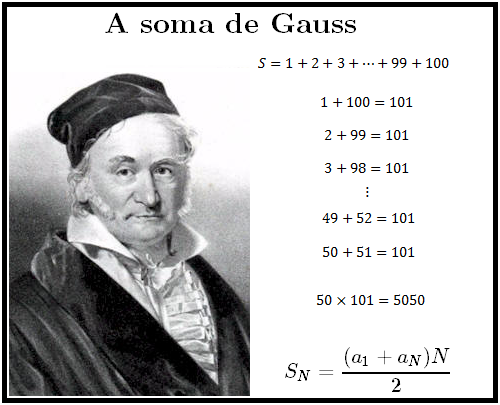
\includegraphics[height=0.5\textwidth, width=0.8\textwidth]{Gauss}
    %\caption{Revista Exame 2017 (\cite{exame17})}
    %\label{figRotulo}
  \end{figure}
\end{block}
\end{frame}

\begin{frame}{}
\frametitle{Cuidado!}
\begin{block}{}
\justifying
\begin{enumerate}
\item ${\displaystyle \sum_{i=m}^{n}a_{i}(x_{i}+k)\neq\sum_{i=m}^{n}(a_{i}x_{i}+k)}$\pause
\item ${\displaystyle \sum_{i=m}^{n}a_{i}(x_{i}+k)\neq\sum_{i=m}^{n}a_{i}x_{i}+k}$\pause
\item ${\displaystyle \sum_{i=1}^{n}a_{i}^{2}\neq \Biggl(\sum_{i=1}^{n}a_{i}\Biggl)^{2}}$ 
\end{enumerate}
\end{block}
\end{frame}

\begin{frame}{}
\frametitle{}
\begin{block}{}
\justifying
{\bf Soma infinita:} é a soma de infinitos termos, a qual, espera-se que convirja para um determinado
valor. É muito aplicada na teoria da probabilidade na definição de modelos em espaços infinitos discretos.
$${\displaystyle \sum_{i=1}^{\infty}x_{i}=x_{1}+x_{2}+\cdots}$$
\end{block}
\end{frame}

\begin{frame}{}
\frametitle{}
\begin{block}{}
\justifying
{\bf Exemplo:} Qual é a fração geradora da dizima $3.55555\cdots$?
\begin{align*}
3.55555\cdots &=3+0.5+0.05+0.005+0.0005+0.00005+\cdots\\
&=3+\dfrac{5}{10}+\dfrac{5}{100}+\dfrac{5}{1000}+\dfrac{5}{10000}+\cdots\\
&=3+{\displaystyle \sum_{i=1}^{\infty}\dfrac{5}{10^{i}}}\\
&=3+\dfrac{5/10}{1-1/10}\\
&=3+\dfrac{5}{9}=\dfrac{32}{9}
\end{align*}
\end{block}
\end{frame}

\section{Produtório}
\begin{frame}{}
\frametitle{}
\begin{block}{}
\justifying
De forma alternativa, como na adição, o produto pode ser escrito usando-se um símbolo de produto, chamado 
produtório $\prod$ que é a letra pi maíuscula no alfabeto grego.
$${\displaystyle \prod_{i=1}^{n}x_{i}=x_{1}x_{2}\cdots x_{n}}$$
\end{block}
\end{frame}

% \begin{frame}{}
% \frametitle{Referências Bibliográficas}
% \bibliography{bibliografia}
% \end{frame}

\end{document} 
